%!TEX root = ../Thesis.tex
\begin{figure}[h]
\centering
\begin{subfigure}[b]{0.45\textwidth}
    \centering
    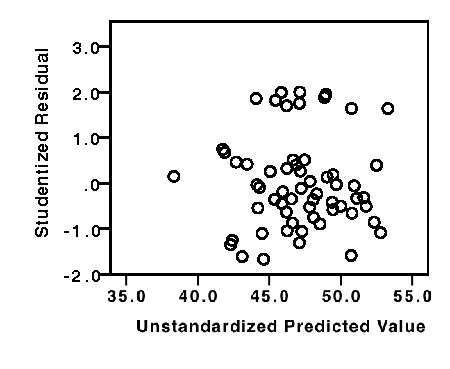
\includegraphics[width=\textwidth]{images/linearity/ValMax.eps}
    \caption{Related to test of valence, maximum pressure, and duration}
    \label{fig:valence_maximum}
\end{subfigure}
\quad
\begin{subfigure}[b]{0.45\textwidth}
    \centering
    \includegraphics[width=\textwidth]{images/linearity/ValAvg.eps}
    \caption{Related to test of valence, average pressure, and duration}
    \label{fig:valence_avg}
\end{subfigure}
\par\bigskip
\par\bigskip
\begin{subfigure}[b]{0.45\textwidth}
    \centering
    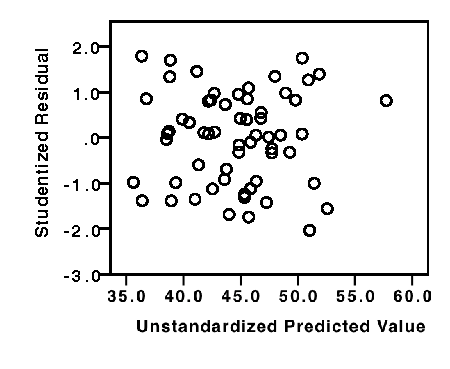
\includegraphics[width=\textwidth]{images/linearity/ArMax.eps}
    \caption{Related to test of arousal, maximum pressure, and duration}
    \label{fig:arousal_maximum}
\end{subfigure}
\quad
\begin{subfigure}[b]{0.45\textwidth}
    \centering
    \includegraphics[width=\textwidth]{images/linearity/ArAvg.eps}
    \caption{Related to test of arousal, average pressure, and duration}
    \label{fig:arousal_avg}
\end{subfigure}
\caption{Scatter plots of predicted values against studentitized residuals. Note that because of random nature, linearity can still be assumed.}
\end{figure}